% LaTeX source for ``การเรียนรู้ของเครื่องสำหรับเคมีควอนตัม (Machine Learning for Quantum Chemistry)''
% Copyright (c) 2022 รังสิมันต์ เกษแก้ว (Rangsiman Ketkaew).

% License: Creative Commons Attribution-NonCommercial-NoDerivatives 4.0 International (CC BY-NC-ND 4.0)
% https://creativecommons.org/licenses/by-nc-nd/4.0/

\chapter{ชุดข้อมูลทางเคมี}
\label{ch:dataset}

%--------------------------
\section{ปริภูมิเคมี}
%--------------------------

ปริภูมิเคมี (Chemical space) 

%--------------------------
\section{ชุดข้อมูลมาตรฐาน}
%--------------------------

QM9 เป็นหนึ่งใน Dataset ที่ได้รับความนิยมมากในสายงานวิจัยเคมีควอนตัม โดยเฉพาะงานวิจัยทางด้าน ML ซึ่งถูกใช้อย่างแพร่หลายตั้งแต่ปี ค.ศ. 
2014 เป็นต้นมา\autocite{ramakrishnan2014} โดยบทความวิจัยชิ้นแรกที่ได้รับการตีพิมพ์นั้นได้รายงานค่าความแม่นยำและความผิดพลาดว่าไม่เกิน 
10 kcal/mol ซึ่งถือว่าเยอะมาก ๆ และต่อมาได้มีการพัฒนาระเบียบวิธีวิจัยรวมไปถึงโมเดล ML และ Descriptor ใหม่ ๆ จนทำให้ในปัจจุบันนั้น%
นักวิจัยสามารถที่จะทำนายหรือพยากรณ์ค่าพลังงานของโมเลกุลทางเคมีอินทรีย์ขนาดเล็กได้แม่นยำมากโดยมีค่าความคลาดเคลื่อนประมาณ 1 kcal/mol 
หรือต่ำกว่านั้น ซึ่งเป็นค่าที่เรียกว่า Chemical Accuracy หรือเทียบเท่ากับค่าความคลาดเคลื่อนของเครื่องมือทดลองทางเคมี

QM9 ประกอบไปด้วยข้อมูลคุณสมบัติอิเล็กทรอนิกส์ของโมเลกุลมากถึง 134,000 โมเลกุล โดยโมเลกุลทั้งหมดนั้นจะเป็นโมเลกุลที่มีธาตุพื้นฐานเป็น%
องค์ประกอบ ประกอบไปด้วย คาร์บอน ไนโตรเจน ออกซิเจน ไฮโดรเจน และฟลูออรีน โดย Feature หลักของ QM9 ก็จะมีพิกัดคาร์ทีเชียนของอะตอม%
ในโมเลกุลซึ่งได้มาจากการคำนวณการปรับโครงสร้างด้วยระเบียบวิธี B3LYP/6-31G(2df,p) และนอกจากนี้ยังมีค่า Label หรือค่าที่ไว้ใช้ในการเปรียบ%
เทียบการพยากรณ์ดังแสดงในตารางที่ \ref{tab:qm9_feature}
\footnote{โมเดล ML ที่เหมาะสมสำหรับการฝึกสอนด้วย QM9 นั้นจะต้องไม่ขึ้นกับ Translation, Rotation และ Permutation}

\begin{table}[H]
    \centering
    \caption{ข้อมูล Feature ของชุดข้อมูล QM9}
    \label{tab:qm9_feature}
    \small
    \begin{tabular}{llll}\toprule
    \textbf{ดัชนี} &\textbf{ชื่อ} &\textbf{หน่วย} &\textbf{คำอธิบาย} \\\midrule
    0 &index &- &Consecutive, 1-based integer identifier of molecule \\
    1 &A &GHz &Rotational constant A \\
    2 &B &GHz &Rotational constant B \\
    3 &C &GHz &Rotational constant C \\
    4 &mu &Debye &Dipole moment \\
    5 &alpha &Bohr$^3$ &Isotropic polarizability \\
    6 &homo &Hartree &พลังงานของ Highest occupied molecular orbital (HOMO) \\
    7 &lumo &Hartree &พลังงานของ Lowest unoccupied molecular orbital (LUMO) \\
    8 &gap &Hartree &Gap (พลังงานระหว่าง LUMO and HOMO) \\
    9 &r2 &Bohr$^2$ &Electronic spatial extent \\
    10 &zpve &Hartree &Zero point vibrational energy \\
    11 &U0 &Hartree &Internal energy at 0 K \\
    12 &U &Hartree &Internal energy at 298.15 K \\
    13 &H &Hartree &Enthalpy at 298.15 K \\
    14 &G &Hartree &Free energy at 298.15 K \\
    15 &Cv &cal/(mol K) &Heat capacity at 298.15 K \\
    \bottomrule
    \end{tabular}
\end{table}

นอกจาก QM9 แล้วยังมีชุดข้อมูลอื่น ๆ ที่นักวิจัยมักจะนำมาใช้ในการฝึกสอนโมเดลและทำวิจัย เช่น QM7\autocite{blum2009,rupp2012a} และ 
QM8\autocite{ruddigkeit2012,ramakrishnan2015} ซึ่งก็จะมี Label สำหรับวัตถุประสงค์ในการฝึกสอนโมเดลในการเพิ่มความสามารถการพยากรณ์%
คุณสมบัติเคมีของโมเลกุลที่ต่างกันออกไป โดยชุดข้อมูลที่กล่าวมาทั้งหมดนั้นสามารถดาวน์โหลดได้ฟรีจากเว็บไซต์ 
\url{http://quantum-machine.org/datasets}

%--------------------------
\section{การสร้างชุดข้อมูล}
\idxth{ชุดข้อมูล!การสร้างชุดข้อมูล}
%--------------------------

ชุดข้อมูลที่ใช้ใน ML นั้นโดยทั่วไปแล้วมักจะมีอยู่ 2 ประเภทคือชุดข้อมูลสำหรับการฝึกสอน (Training Set) และชุดข้อมูลสำหรับการทดสอบ 
(Test Set) ซึ่งวัตถุประสงค์ของชุดข้อมูลทั้งสองประเภทนี้ก็ตรงตัวเลยก็คือ Training Set จะถูกนำมาใช้ในการฝึกสอนโมเดล ส่วน Test Set 
จะถูกเก็บไว้ใช้ในการทดสอบโมเดลหรือการทำนายคำตอบที่โมเดลถูกสอนมา (Prediction) อย่างไรก็ตาม การฝึกสอนโมเดลโดยการใช้ Train Set 
ทั้งหมดนั้นมักจะทำให้เกิดความโน้มเอียง (Bias) ที่เกิดขึ้นจากชุดข้อมูลและส่งผลให้เกิด Biased ในขั้นตอน Prediction ด้วย เพราะป้องกันเหตุการณ์%
ดังกล่าวและทำให้เกิด Bias น้อยที่สุด เรามักจะทำการแบ่ง (Split) ชุดข้อมูลฝึกสอนให้เป็นชุดข้อมูลสำหรับการฝึกสอนจริง ๆ (Actual Training 
Set) และชุดข้อมูลสำหรับการตรวจสอบและยืนยันความถูกต้องซึ่งเรียกอีกอย่างว่า Validation Set

\begin{figure}[H]
    \centering
    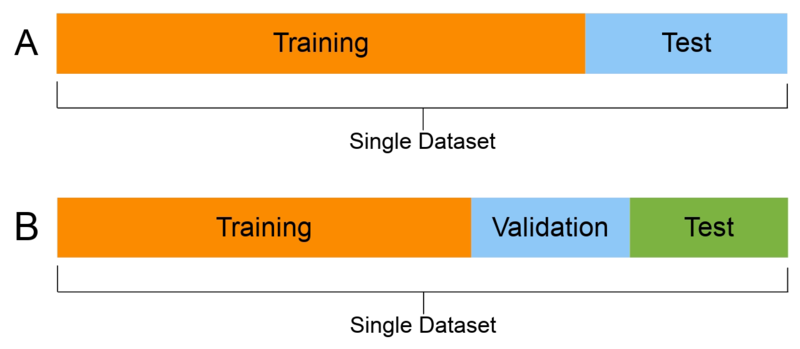
\includegraphics[width=0.8\linewidth]{fig/dataset.png}
    \caption{การแบ่งชุดข้อมูลทั้งหมดออกเป็น (A) Training Set และ Test Set และ (B) Training Set, Validation Set และ 
    Test Set (เครดิตภาพ: Wikimedia Commons)}
    \label{fig:dataset}
\end{figure}

ภาพที่ \ref{fig:dataset} แสดงสัดส่วนแบบคร่าว ๆ ในการแบ่งชุดข้อมูลออกเป็น Training Set และ Test Set และแสดงการแบ่งชุดข้อมูล%
อีกครั้งให้เป็น Training Set ที่จะถูกนำไปใช้ในการฝึกสอนโมเดลจริง ๆ และ Validation Set ที่จะถูกนำมาทดสอบโมเดลเพื่อเป็นการหยั่งเชิง%
ความสามารถของโมเดลก่อนที่จะนำไปใช้ทำนายค่าของ Test Set\footnote{โดยทั่วไปแล้วหลาย ๆ คนมักจะทำการแบ่งโดยใช้อัตราส่วนคือ 
80\% และ 20\% ตามหลักการของ Pareto \url{https://en.wikipedia.org/wiki/Pareto_principle}}

แล้วขั้นตอนการลด Bias นั่นมันเกิดขึ้นได้อย่างไร คำตอบก็คือในการแบ่งข้อมูลออกมาเป็น Validation Set (เช่นแบ่งออกมา 20\% จากทั้งหมด)
โดยทำการสุ่มเลือกบางส่วนของข้อมูลออกมา ซึ่งถ้าหากเราทำวนไปแบบนี้ไปเรื่อย ๆ เราจะเรียกว่าเป็นการทำ Validation แบบข้ามไปมาทั่วทั้ง 
Training Set ซึ่งเมื่อเรานำ Training Set แต่ละชุดไปฝึกสอนโมเดล เราจะได้ประสิทธิภาพของโมเดลแบบเฉลี่ย เปรียบเสมือนเป็นการเกลี่ย% 
หาความเท่ากันของข้อมูลนั่นเอง (กระจายออกไปให้เสมอกัน) ท้ายที่สุดแล้วถ้าเราแบ่งชุดข้อมูลตามที่ได้อธิบายมา เราจะมีอัตราส่วนของชุดข้อมูล%
ย่อย ๆ แต่ละประเภท ดังนี้

\begin{itemize}
    \item Training: 60\%
    \item Cross Validation: 20\%
    \item Testing: 20\%
\end{itemize}

%--------------------------
\subsection{ขั้นตอนการสร้างชุดข้อมูล}
\idxth{ชุดข้อมูล!ขั้นตอนการสร้างชุดข้อมูล}
%--------------------------


%--------------------------
\subsection{การสร้างชุดข้อมูลเคมีควอนตัม}
\idxth{ชุดข้อมูล!การสร้างชุดข้อมูลเคมีควอนตัม}
%--------------------------
